% !TEX root = ../../../main/aws_chabauty.tex
\newpage
\subsection{Lecture 3}

	\begin{figure}[!ht]
	\centering
	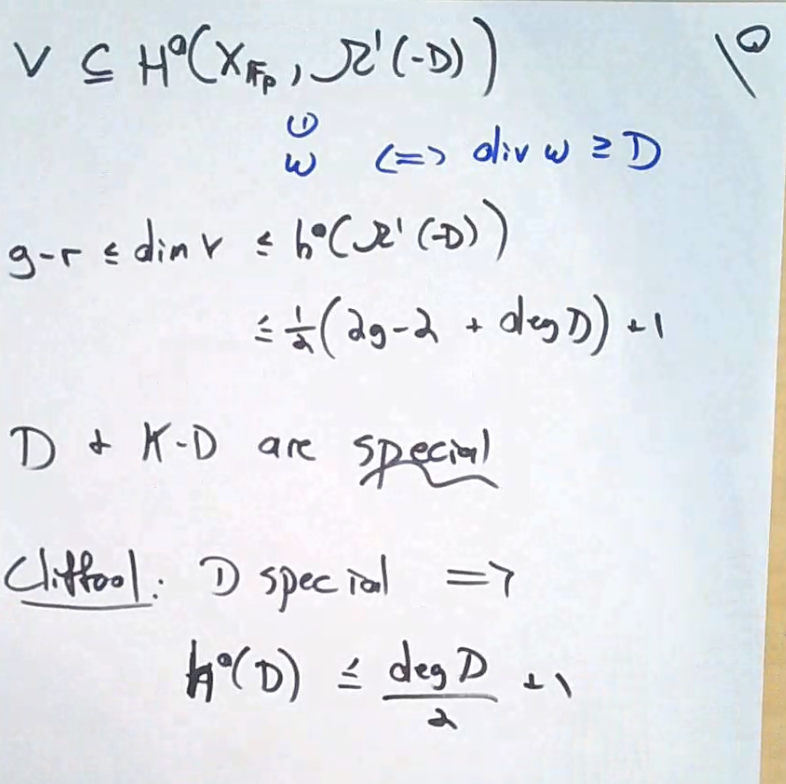
\includegraphics[width=0.5\textwidth]{../images/im17.png}
	\end{figure}
	
	\begin{figure}[!ht]
	\centering
	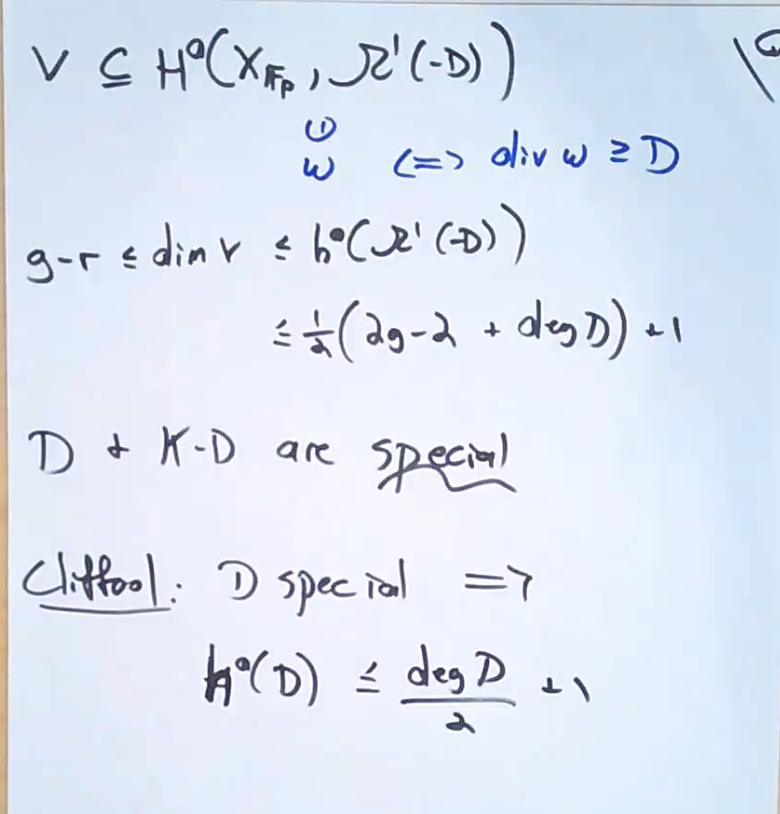
\includegraphics[width=0.5\textwidth]{../images/im18.png}
	\end{figure}
	
$|D|= \{ E \geq 0 \colon E \cap D \} \simeq \P^r$.

	\[
	\begin{aligned}
	r(D)&= -1 \quad \text{if } |D|= \emptyset \\
	r(D)&= 0 \quad \text{if } |D|\neq \emptyset \\
	r(D)&= 1 \quad \text{if } \forall P \in X, |D - P| \neq \emptyset \\
	r(D)&\geq i \quad \text{if } \forall E \geq 0 \text{ of deg }E \leq i, |D - E|\neq \emptyset 
	\end{aligned}
	\]
Then $X$ sm, then $r(D)= \dim H^0(X,D)-1$. If $X$ is singular, then $r(D) \neq \dim H^0(D)$


	\begin{figure}[!ht]
	\centering
	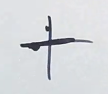
\includegraphics[width=0.2\textwidth]{../images/im19.png}
	\end{figure}


The rank of $D$ is semicontinuous, i.e. if $\fX/E_P$, then $\fX_{\Qp} \to \fX_{\F_p}$ then $r(D) \geq r(D')$ [Hartshorne III.12]. 


	\begin{figure}[!ht]
	\centering
	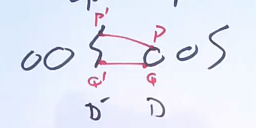
\includegraphics[width=0.4\textwidth]{../images/im20.png}
	\end{figure}


\begin{rem}
This inequality can be strict. If $P,Q \in X$ are not hyperelliptic, then reduces to $P',Q'= i(P)$, $h^0(P+Q)= 1$ and $h^0(P' + i(P))= 2$.
\end{rem}


\begin{dfn}[Regular]
Let $X$ be a scheme. We say that $X$ is regular if for all $P \in X$ corresponding to $\p$, we have $\dim_{k(\p)} \p/\p^2= \dim X$.
\end{dfn}


\begin{ex}
$y^2 - x^3- p/\Z_p$. 
	\[
	\begin{tikzcd}
	\fX \arrow{d}{\text{not sm}} \\
	\spec \Z_p
	\end{tikzcd}
	\]
$\fX$ is regular, $\fm= (x,y,p)$, $\fm/\fm^2= \langle x,y,p \rangle= \langle x,y \rangle$ PGM
\end{ex}


	\begin{figure}[!ht]
	\centering
	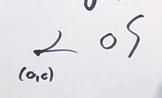
\includegraphics[width=0.2\textwidth]{../images/im21.png}
	\end{figure}


If $\fX/\Z_p$ is a regular proper model of a sm curve
	\[
	\im( \fX(\Qp) \ma{\text{red}} \fX(\F_p) ) \subseteq \fX^{\text{sm}}(\F_p)
	\]


\begin{ex}
$y^2 - x^3 - p$, $[0,0]= \emptyset$, $y^2 - x^3 - p^2$, $[0,0]$ ? lop

Lorenzini-Tucker, Mc Poonen

regular, etc, $\fX$ r.p. model
	\[
	\#X(\Q) \leq \#\fX(\F_p) + 2g-2
	\]
The idea is the same proof:

	\begin{figure}[!ht]
	\centering
	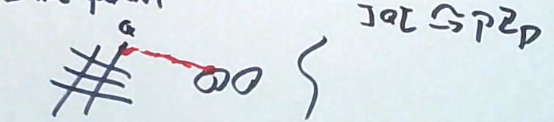
\includegraphics[width=0.5\textwidth]{../images/im22.png}
	\end{figure}
\end{ex}




\subsubsection{Matt Baker's Idea: Degenerate Even More}


	\begin{figure}[!ht]
	\centering
	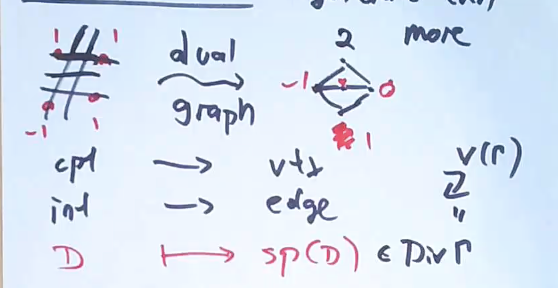
\includegraphics[width=0.5\textwidth]{../images/im23.png}
	\end{figure}



Baker, Baker-Norine

Notion of linear system, equivalence of divisors, and notion of rank, i.e. $|D|, r(D)$, $r(D) \leq r(\sp(D))$
	\[
	K_P= \sum (\deg v - 2)[v]
	\]
Notion of special RR and Clifford 


For Riemann-Roch, we have $r(D) - r(K_P - D)= \deg D + 1 - g$. Clifford gives if $D$ is special, then $r(D) \leq \frac{\deg D}{2}$. 


\begin{thm}[Katz,ZB]
Suppose $\fX$ is a regular proper model and $\fX_{\F_p}$ is totally degenerated. Then $\sp(D_{\text{ch}})$ is special
	\[
	D_{\text{ch}}= \sum n_\Q[\Q]
	\]
Actually, $r(K_P - D) \geq g - r - 1$.
\end{thm}

\pf (of rank favorability) $g - r - 1 \leq r(K_r - \sp(D)) \leq \frac{\deg(K_r - \deg D)}{2}= \frac{1}{2} (2g - 2 + \deg D)$. \qed \\



\subsubsection{Chip Firing}

Goal: Get (everybody) out of debt. 


	\begin{figure}[!ht]
	\centering
	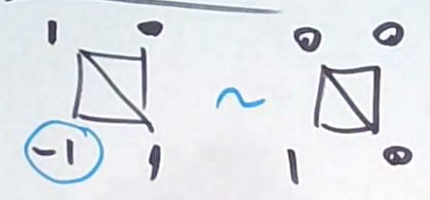
\includegraphics[width=0.5\textwidth]{../images/im24.png}
	\end{figure}
	
	\begin{figure}[!ht]
	\centering
	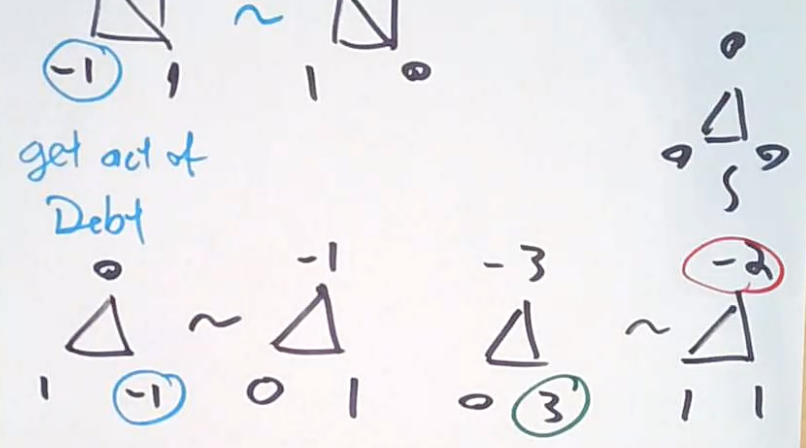
\includegraphics[width=0.5\textwidth]{../images/im25.png}
	\end{figure}


We say that $D \sim D^1$ if they differ by some sequence of loans and borrows. $\text{component group of special fiber of neron model } \simeq \pic^0 \Gamma \subseteq \pic \Gamma= \div \Gamma/\sim$.


$|D|= \{ D' \geq 0 \colon D' \sim D \}$. $r(D) \geq i$ if for all $E \geq 0$ with $\deg E \leq i$, $|D - E|\neq \emptyset$. 


	\begin{figure}[!ht]
	\centering
	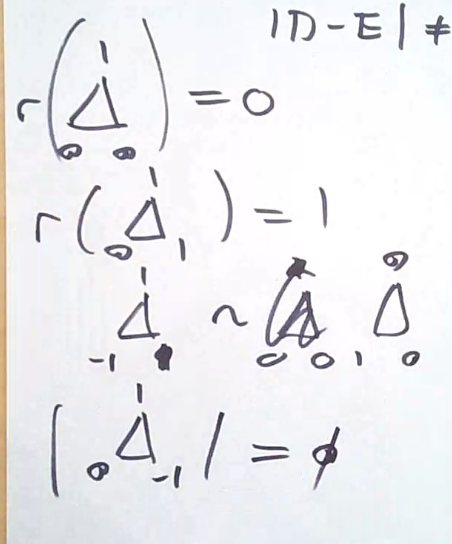
\includegraphics[width=0.5\textwidth]{../images/im26.png}
	\end{figure}


$\fX/\Z_p$, $\fX_{\F_p}= \cup C_i$, $\pic \fX \ma{\sp} \div \Gamma'$ given by $L \mapsto \sp(L):= \sum (\deg L \big|_{C_i})[v_i]$.

	\begin{figure}[!ht]
	\centering
	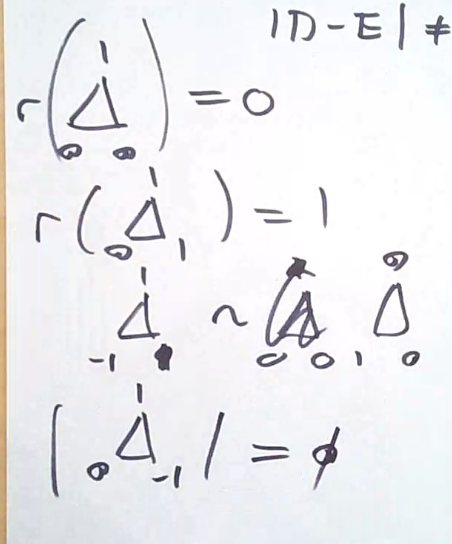
\includegraphics[width=0.5\textwidth]{../images/im26.png}
	\end{figure}


\begin{ex}
$L= \O(C_i)$
	\[
	\deg \O(C_i) \big|_{C_j}=
	\begin{cases}
	\# \text{ int points of } C_i \cap C_j \\
	\# \text{ self int of } C_i
	\end{cases}
	\]
$\fX_{\F_p}= (P)$ then $C_i \sim - \sum_{j \neq i} C_j$

$\sp(\O(C_i))$ if and only if firing at vertex $i$.
\end{ex}


\begin{ex}
$L= \omega_Z$.

Adjunction: $(\omega_\fX \otimes \O(C_i)) \big|_{C_i} \simeq \Omega^1_{C_i}$
	\[
	\begin{aligned}
	\deg \omega_\fX \big|_{C_i}&= \deg \Omega^1_{\P^1} - \deg \O(C_i) \big|_C \\
	&= -2 + \#\text{ int points of }C_i \text{ with rest }\fX \\
	&= K_p
	\end{aligned}
	\]

	\begin{figure}[!ht]
	\centering
	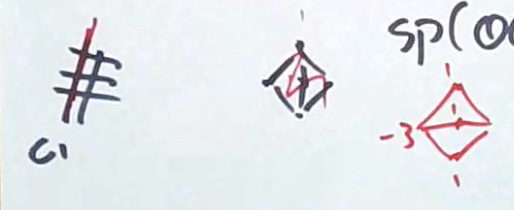
\includegraphics[width=0.5\textwidth]{../images/im28.png}
	\end{figure}
\end{ex}


As an upshot,

	\begin{figure}[!ht]
	\centering
	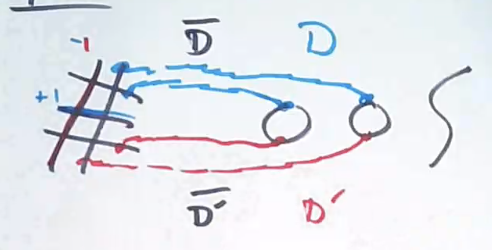
\includegraphics[width=0.5\textwidth]{../images/im29.png}
	\end{figure}

$D \sim D'$ on $\fX_{\sp}$, $\div f= D - D'$, $f: \fX_{\sp} \to \P^1$, extend $f$ to $\fX \leftrightarrow F$. Then $\div F= \ov{D} - \ov{D}' + \sum \alpha_i C_i$. The equivalence $\sp(\ov{D})$ with $\sp(\ov{D}')$ is witnessed by lending at $C_i(v_i)$ $\alpha_i$ many times. 


	\begin{figure}[!ht]
	\centering
	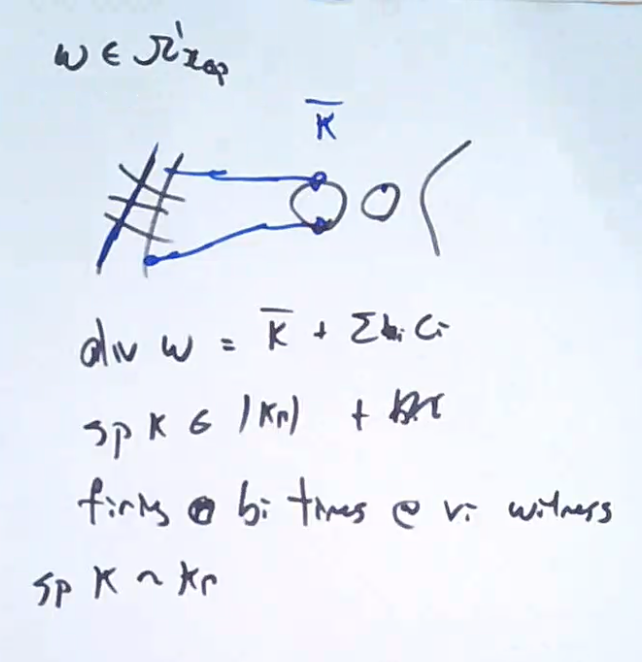
\includegraphics[width=0.5\textwidth]{../images/im30.png}
	\end{figure}




























